\section{Implementierung des \acs{YARN}"=Modells}
\label{sec:yarnModel}

Das implementierte \ac{YARN}"=Modell besteht, wie bereits in \cref{sec:modelArchitecture} gezeigt, aus fünf Komponenten und den Komponentenfehlern der hier relevanten \ac{YARN}"=Komponenten.
Die vier implementierten \ac{YARN}"=Komponenten sind die Anwendungen, ihre Attempts und Container, sowie die Nodes.
Zudem wurde eine Klasse implementiert, die zur Repräsentation des \ac{RM} dient, und als Controller im Rahmen des Testens mit \ac{ss} dient.
Einen Überblick über den Aufbau des implementierten \ac{YARN}"=Modells gibt folgendes Klassendiagramm:

\begin{figure}[h]
    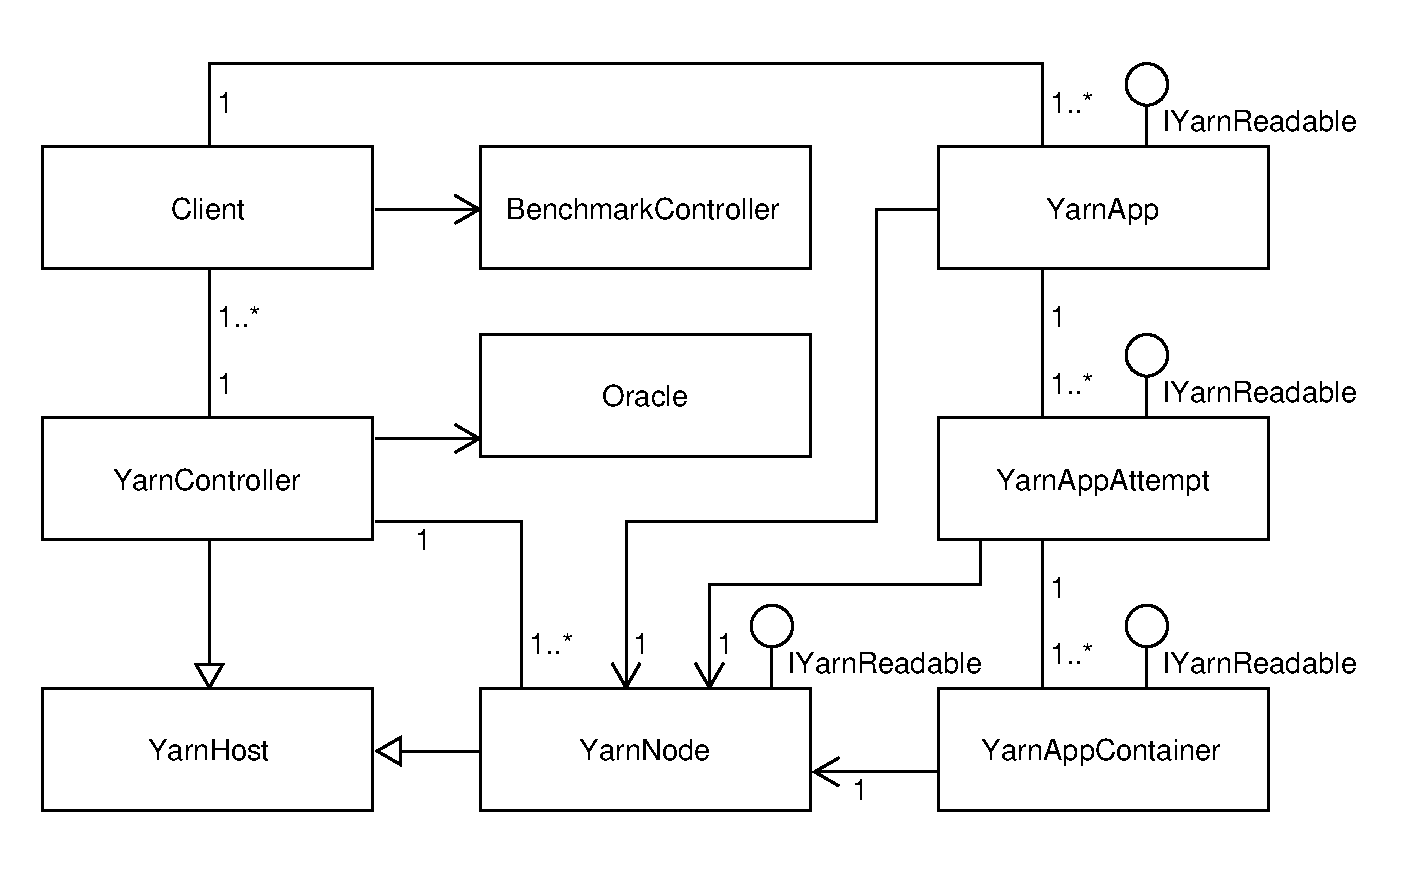
\includegraphics{./resources/yarnModel_ls_MA.pdf}
    \caption[Grundlegender Aufbau des \acs{YARN}"=Modells]
        {Grundlegender Aufbau des \acs{YARN}"=Modells.
        Assoziationen und weitere Verbindungen zum Treiber und \acs{ss} sind hier aus Gründen der Übersichtlichkeit nicht dargestellt.}
    \label{fig:yarnModelClassDiagram}
\end{figure}

Zunächst werden im Folgenden die relevanten \ac{YARN}"=Komponenten mit ihren Komponentenfehlern erläutert, von denen für diese Fallstudie nicht alle vier benötigt wurden, anschließend die anderen Komponenten des \ac{YARN}"=Modells.

\subsection{Relevante \acs{YARN}"=Komponenten}
\label{sec:yarnComponents}

Die vier implementierten, relevanten \ac{YARN}"=Komponenten sind die Anwendungen, ihre Attempts und Container sowie die Nodes des Clusters.
Obwohl die die Anwendungs"=Container in dieser Fallstudie nicht benötigt werden, waren sie für die in \cite{Eberhardinger2018} beschriebene Fallstudie notwendig, welche ebenfalls mit dem hier beschriebenen Modell durchgeführt wurden.

\subsubsection{Übersicht der implementierten Komponenten}
\label{subsec:yarnComponentsOverview}

Eine Übersicht über die Implementierung der \ac{YARN}"=Komponenten gibt folgendes Klassendiagramm:

\begin{figure}[h]
    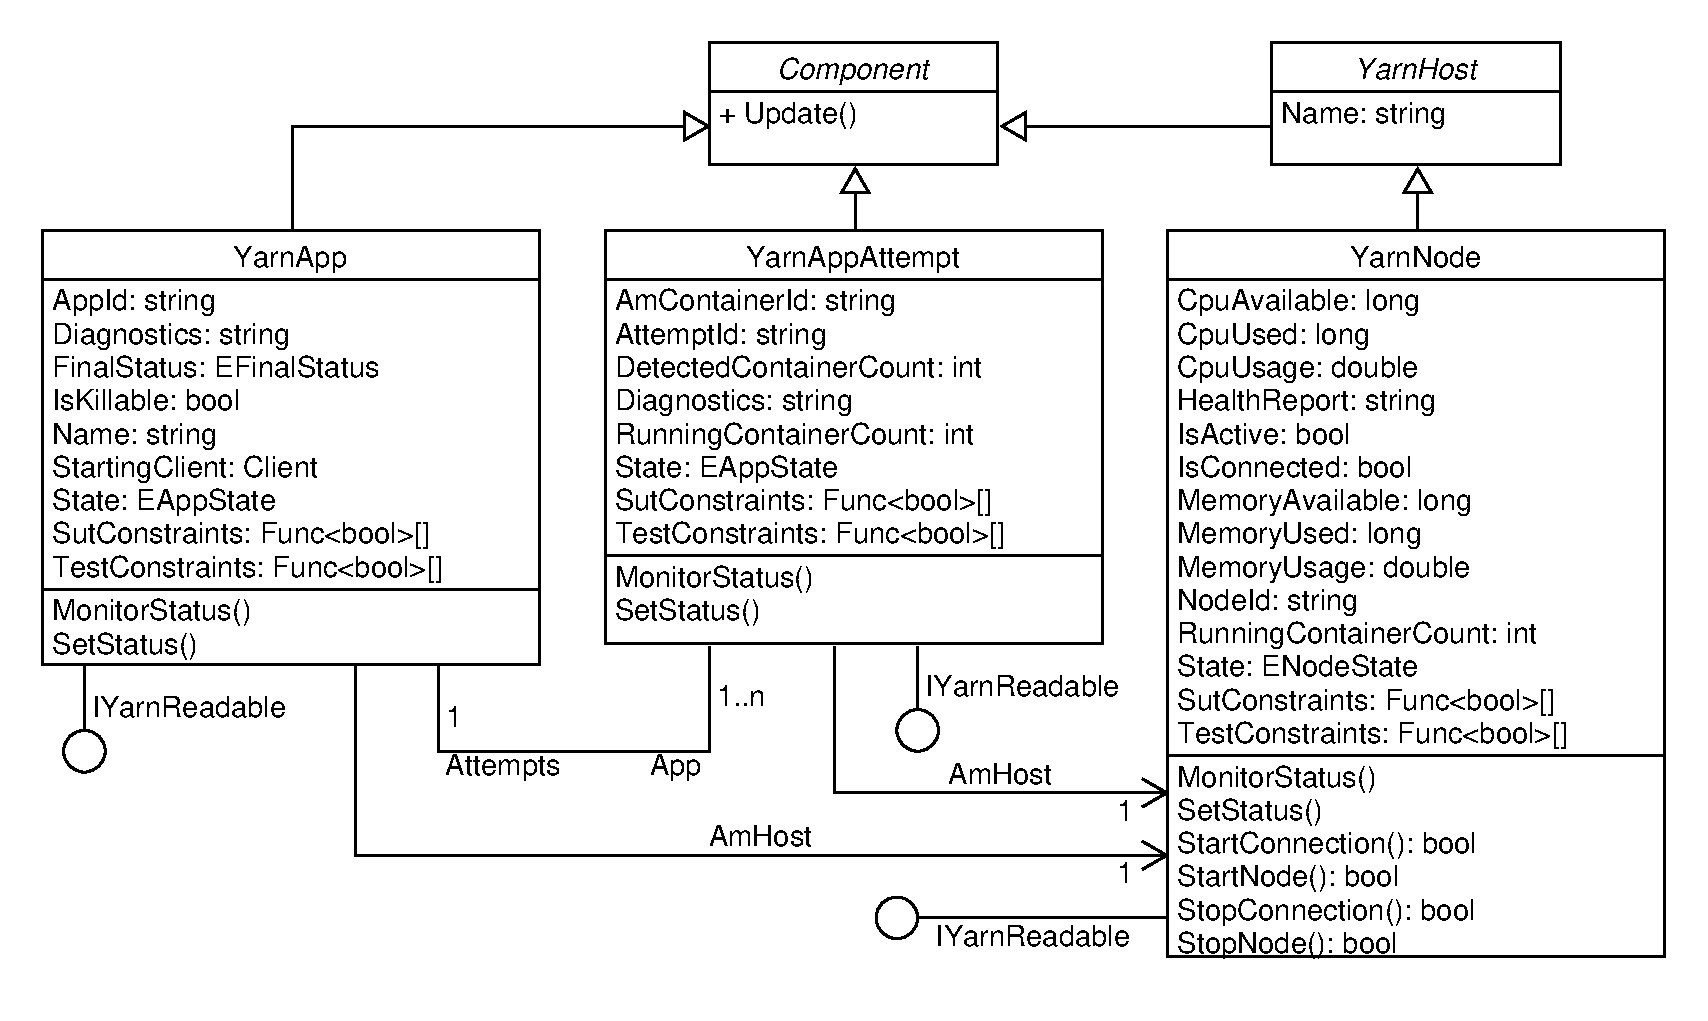
\includegraphics[width=\columnwidth]{./resources/yarnComponents.pdf}
    \caption[Für die Fallstudie relevante, implementierte \acs{YARN}"=Komponenten mit den wichtigsten Eigenschaften und Methoden]
        {Für die Fallstudie relevante, implementierte \acs{YARN}"=Komponenten mit den wichtigsten Eigenschaften und Methoden.
        Dies sind alle für die spätere Durchführung und zur Ausgabe des Zustandes (vgl. \cref{subsec:dataOrganisation}) wichtigen Eigenschaften und Methoden.
        Aus Gründen der Übersichtlichkeit sind die implementierten Komponentenfehler, einige der \texttt{IYarnReadable} bereitgestellten, relevanten Eigenschaften und Methoden, sowie die Klasse \texttt{YarnAppContainer} nicht aufgeführt.}
    \label{fig:yarnComponentsClassDiagram}
\end{figure}

Die Eigenschaft \texttt{AmHost} speichert den ausführenden Node des \ac{AppMstr} der Anwendung bzw. des Attempts, die Eigenschaft \texttt{IsKillable} gibt an, ob eine Anwendung derzeit ausgeführt ist und somit vorzeitig abgebrochen werden kann.
Die Eigenschaften \texttt{Diagnostics} bzw. \texttt{HealthReport} stellen von Hadoop zur Verfügung gestellte weitere Informationen bei Fehlern dar.
Die \texttt{State}"=Eigenschaften bzw. \texttt{FinalState} speichern die von Hadoop angegebenen Zustände der \ac{YARN}"=Komponenten.
Hierfür wurden entsprechende Auflistungen basierend auf den in \cite{HadoopRmApi271} angegebenen möglichen Werten für die jeweiligen Zustände im Modell implementiert.

Da für diese Fallstudie die Daten der Container selbst nicht relevant sind, wird im hier verwendeten Modell nur gespeichert, wie viele Anwendungs"=Container beim Monitoring im aktuellen Testfall (\texttt{RunningContainerCount}) bzw. für alle bisher ausgeführten Testfälle kumuliert (\texttt{DetectedContainerCount}) erkannt wurden.
Für die Tests in \cite{Eberhardinger2018} werden die Daten der Container genauso wie die der anderen \ac{YARN}"=Komponenten gespeichert.
Hierfür enthalten die Klassen \texttt{YarnAppAttempt} und \texttt{YarnAppContainer} entsprechende Eigenschaften zur jeweiligen Zuordnung analog zu denen zwischen \texttt{YarnApp} und \texttt{YarnAppAttempt}.
Die Eigenschaft \texttt{AmContainerId} speichert zudem die Container"=ID des \ac{AppMstr}"=Containers.

Die Eigenschaften mit dem Präfix \texttt{CPU} bzw. \texttt{Memory} in \texttt{YarnNode} dienen zur Speicherung der derzeitigen Auslastung der CPU"=Kerne bzw. des Speichers eines Nodes.
Benötigt werden diese Werte zur in \cref{subsubsec:simulationFaultActivation} beschriebenen Berechnung, ob ein Komponentenfehler aktiviert oder deaktiviert wird.

Die Eigenschaften \texttt{SutConstraints} und \texttt{TestConstraints} sowie die Methoden \texttt{MonitorStatus()} und \texttt{SetStatus()} werden von \texttt{IYarnReadable} bereitgestellt und speichern die Constraints bzw. dienen zur Durchführung des Monitorings der implementierten Komponenten.
Die Start"= und Stop"=Methoden sowie die Eigenschaften \texttt{IsActive} und \texttt{IsConnected} in \texttt{YarnNode} dienen zur Identifikation und Injizierung bzw. Reparieren der Komponentenfehlern.
Diese Eigenschaften und Methoden werden daher auf den folgenden Seiten näher beschrieben.

Neben den dargestellten, relevanten Eigenschaften und Methoden wurden zahlreiche weitere implementiert, welche einerseits zur Vollständigkeit der implementierten Komponenten für die Tests in \cite{Eberhardinger2018}, andererseits auch zur Ausführung mithilfe des \ac{ss}"=Frameworks benötigt werden.
Letztere sind \zB zur Speicherung von Strings notwendig, welche aufgrund der Einschränkungen von \ac{ss} (vgl. \cref{sec:ssharp}) nicht jederzeit frei genutzt werden können.
Strings sind im \ac{YARN}"=Modell daher zur Speicherung immer als  \texttt{char}"=Arrays implementiert, werden jedoch zur einfacheren Nutzung im Modell in Strings konvertiert:

\begin{lstlisting}[label=lst:modelCharArrayAsString,style=cs,
caption={[Implementierung der Eigenschaft AppId]
    Implementierung der Eigenschaft \texttt{AppId}.
    Die beiden Methoden \texttt{GetCharArrayAsString} und \texttt{SetCharArrayOnString} führen die Konvertierung in den \texttt{char}"=Array bzw. des \texttt{char}"=Arrays in einen String durch.}]
public char[] AppIdActual { get; }

[NonSerializable]
public string AppId
{
  get { return ModelUtilities.GetCharArrayAsString(AppIdActual); }
  set { ModelUtilities.SetCharArrayOnString(AppIdActual, value); }
}
\end{lstlisting}

Die \texttt{Update()}"=Methoden starten bei allen vier implementierten \ac{YARN}"=Komponenten die jeweiligen Monitoring"=Funktionen, bei \texttt{YarnNode} werden zudem \texttt{StartNode()} und \texttt{StartConnection()} ausgeführt um mögliche zuvor injizierte Komponentenfehler im realen Cluster zu reparieren.

Da bei der Ausführung des Modells durch \ac{ss} keine neuen Instanzen erzeugt werden können (vgl. \cref{sec:ssharp}), dienen die jeweiligen IDs der Komponenten auch als Indikator, ob die jeweilige Komponenten"=Instanz derzeit benötigt wird und somit Daten gespeichert werden sollen.
Daher wird das Monitoring auch nur dann ausgeführt, wenn der Instanz eine nicht leere ID \zB in Form der \texttt{AppId} zugewiesen wurde.

\subsubsection{Implementierung der Komponentenfehler}
\label{subsubsec:yarnComponentFaults}

Die im \ac{YARN}"=Modell implementierten Komponentenfehler wurden direkt in den entsprechenden \ac{YARN}"=Komponenten implementiert.
Implementiert wurden hierbei mit \texttt{NodeDeadFault} und \texttt{NodeConnectionErrorFault} zwei jeweils als \texttt{TransientFault} definierte Komponentenfehler für die durch \texttt{YarnNode} repräsentierten Nodes.
Während durch \texttt{NodeDeadFault} der komplette Node beendet wird, trennt \texttt{NodeConnectionErrorFault} nur die Verbindung des Nodes zum Cluster.
Die dazugehörigen Effekt"=Klassen der Komponentenfehler sind jeweils als innere Klassen in \texttt{YarnNode} implementiert.

Die Injizierung und das Reparieren der beiden Fehler geschieht mithilfe der vier Stop- bzw. Start"=Methoden wie \zB \texttt{StopNode()}, die bereits im Klassendiagramm in \cref{fig:yarnComponentsClassDiagram} zu sehen sind.
Wenn ein Komponentenfehler durch das Framework aktiviert wird, wird durch die Effekt"=Klasse die jeweilige Stop"=Methode aufgerufen und so der Fehler injiziert:

\begin{lstlisting}[label=lst:faultInjection,,style=cs,
caption={[Injizierung des Komponentenfehlers NodeDeadFault]
    Injizierung des Komponentenfehlers \texttt{NodeDeadFault} (gekürzt).
    Sollte der Node nicht beendet werden, wird die Injizierung einmalig erneut versucht.
    \texttt{CmdConnector.Faulting} stellt die zur Injizierung verwendete SSH"=Verbindung dar.}]
public class YarnNode : YarnHost, IYarnReadable
{
  [NodeFault]
  public readonly Fault NodeDeadFault = new TransientFault();
  public IHadoopConnector FaultConnector { get; set; }
  
  public bool StopNode(bool retry = true)
  {
    if(IsActive)
    {
      var isStopped = FaultConnector.StopNode(Name);
      if(isStopped)
        IsActive = false;
      else if(retry)
        StopNode(false); // try again once
    }
    return !IsActive;
  }
  
  [FaultEffect(Fault = nameof(NodeDeadFault))]
  public class NodeDeadEffect : YarnNode
  {
    public override void Update()
    {
      StopNode();
    }
  }
}

public class CmdConnector : IHadoopConnector
{
  private SshConnection Faulting { get; }
  
  public bool StopNode(string nodeName)
  {
    var id = DriverUtilities.ParseInt(nodeName);
    Faulting.Run($"{Model.HadoopSetupScript} hadoop stop {id}", IsConsoleOut);
    return !CheckNodeRunning(id);
  }
}
\end{lstlisting}

Das Reparieren von Komponentenfehlern geschieht analog hierzu.
Hierfür werden in der \texttt{Update()}"=Methode die beiden Start"=Methoden aufgerufen, die einen Fehlerhaften Node reparieren.
Eine Besonderheit bildet hierbei die Reparatur des Komponentenfehlers \texttt{NodeConnectionErrorFault}, bei der der Node komplett neu gestartet wird, da es sonst passieren kann, dass der wieder ans Netzwerk angebundene Node sich nicht mit dem \ac{RM} verbindet.

Ob ein Komponentenfehler in einem Testfall aktiviert wird, entscheidet sich anhand der Auslastung des Nodes.
Hierfür sind beide Komponentenfehler mit dem Attribut \texttt{NodeFault} versehen, mit dessen Hilfe entschieden wird, ob ein Komponentenfehler aktiviert oder deaktiviert und somit injiziert bzw. repariert wird.
Der Entscheidungsprozess hierfür ist in \cref{subsubsec:simulationFaultActivation} beschrieben.

Da beide Fehler zudem auch gleichzeitig aktiviert werden können, wurde \texttt{NodeDead""Fault} mithilfe entsprechender \ac{ss}"=Funktionen eine höhere Priorität vergeben, wodurch dieser Vorrang vor dem anderen Komponentenfehler erhält.
Dadurch wird in solchen Fällen der Node beendet und nicht zunächst noch vom Netzwerk getrennt.

Zur einfachen Identifikation der aktiven Komponentenfehler dienen die beiden Eigenschaften \texttt{IsActive} und \texttt{IsConnected}.
In \cref{lst:faultInjection} wird bereits die Auswirkung der beiden Eigenschaft gezeigt, indem verhindert wird, dass ein möglicherweise bereits injizierter bzw. reparierter Komponentenfehler erneut injiziert bzw. repariert wird.
Sie dienen aber auch zur Validierung der Constraints, bei denen mithilfe der beiden Eigenschaften geprüft wird, ob ein Node korrekt als aktiv bzw. defekt erkannt wurde.

\subsubsection{Interface IYarnReadable}
\label{subsubsec:yarnComponentInterface}

Das Interface \texttt{IYarnReadable} ist das zentrale Erkennungsmerkmal der im Modell abgebildeten und implementierten \ac{YARN}"=Komponenten.
Es dient zum einen zur Identifikation aller implementierten \ac{YARN}"=Komponenten, andererseits stellt es auch Eigenschaften und Methoden bereit, welche einerseits dem Testen in \ac{ss} dienen, primär aber dem Ermitteln der Daten aus dem realen Cluster:

\begin{itemize}
    \item \texttt{GetId()}
    \item \texttt{StatusAsString()}
    
    \item \texttt{Parser}
    \item \texttt{IsSelfMonitoring}
    \item \texttt{MonitorStatus()}
    \item \texttt{SetStatus()}
    
    \item \texttt{PreviousParsedComponent}
    \item \texttt{CurrentParsedComponent}
    \item \texttt{SutConstraints}
    \item \texttt{TestConstraints}
\end{itemize}

Die beiden erstgenannten Methoden dienen primär zu Debugging"=Zwecken und zur Rückgabe der ID bzw. der Werte aller Eigenschaften der Komponente als ein String.

Die nachfolgenden vier Eigenschaften und Methoden dienen zum Monitoring der entsprechenden \ac{YARN}"=Komponenten.
Während die Eigenschaft \texttt{Parser} den zu verwendenden Parser (vgl. \cref{subsec:implementedParsers}) speichert, dient die Eigenschaft \texttt{IsSelfMonito""ring} zur Unterscheidung, ob die Daten einer Komponente von dieser selbst ermittelt werden oder dies die übergeordnete Komponente durchführt.
Diese Unterscheidung ist nötig, da \ac{YARN} zwei unterschiedliche Möglichkeiten zur Ermittlung der Daten bietet, die Rückgabe der Daten durch die Kommandozeile oder mithilfe der REST"=API.
Ausführlichere Informationen zu den beiden Varianten sind in \cref{sec:sshDriver} zu finden.
Bei der Nutzung der Kommandozeile zur Ermittlung der Daten eignet sich daher die Selbstermittlung der Daten besser, während bei der Nutzung der Rest"=API die Ermittlung der Daten durch die übergeordnete Komponente geeigneter ist.
Aus diesem Grund ist auch die Methode \texttt{SetStatus()} definiert, da hier unabhängig von der Datenermittlung der aktuelle Status der Komponente abgespeichert werden kann.
Die Durchführung des Monitoring findet in beiden Fällen jedoch mithilfe der Methode \texttt{MonitorStatus()} statt:

\begin{lstlisting}[label=lst:monitorAppStatus,style=cs,
caption={[Implementierung der Methode MonitorStatus() in der Klasse YarnApp]
    Implementierung der Methode \texttt{MonitorStatus()} in der Klasse \texttt{YarnApp} (gekürzt).
    Das Monitoring der anderen Komponenten erfolgt analog hierzu.}]
public void MonitorStatus()
{
  if(IsSelfMonitoring)
  {
    var parsed = Parser.ParseAppDetails(AppId);
    if(parsed != null)
    SetStatus(parsed);
  }
  
  var parsedAttempts = Parser.ParseAppAttemptList(AppId);
  foreach(var parsed in parsedAttempts)
  {
    // search free attempt
    attempt.IsSelfMonitoring = IsSelfMonitoring;
    if(IsSelfMonitoring)
      attempt.AttemptId = parsed.AttemptId;
    else
    {
      attempt.SetStatus(parsed);
      attempt.MonitorStatus();
    }
  }
}
\end{lstlisting}

Die vier restlichen Eigenschaften und Methoden dienen zur Auswertung der Komponente durch \ac{ss}.
Die beiden Eigenschaften \texttt{SutConstraints} und \texttt{TestConstraints} dienen zur Implementierung der in \cref{sec:requirements} definierten Anforderungen in Form von Constraints.

\subsubsection{Constraints der \acs{YARN}"=Komponenten}
\label{subsubsec:yarnComponentConstraints}

Einige der in \cref{sec:requirements} definierten Anforderungen an das \ac{SuT} und gesamte Testsystem sind auch für die \ac{YARN}"=Komponenten relevant.
Die relevanten Bestandteile der Anforderungen für die jeweiligen Komponenten sind mithilfe der beiden in \texttt{IYarnReadable} definierten Eigenschaften \texttt{SutConstraints} und \texttt{TestConstraints} implementiert.
Realisiert sind die beiden Eigenschaften für die Constraints jeweils als \texttt{Func<bool>[]}:

\begin{lstlisting}[label=lst:constraintDefinition,style=cs,
caption={[Definition der Constraints in YarnApp]
    Definition der Constraints in \texttt{YarnApp} (gekürzt)}]
public Func<bool>[] SutConstraints => new Func<bool>[]
{
  // task will be completed if not canceled
  () =>
  {
    if(FinalStatus != EFinalStatus.FAILED)
      return true;
    if(!String.IsNullOrWhiteSpace(Name) &&
        Name.ToLower().Contains("fail job"))
      return true;
    return false;
  },
  // configuration will be updated
};

public Func<bool>[] TestConstraints => new Func<bool>[]
{
  // current state is detected and saved
  () =>
  {
    var prev = PreviousParsedComponent as IApplicationResult;
    var curr = CurrentParsedComponent as IApplicationResult;
    // compare prev, curr and this and return the result
    // or otherwise
    return false;
  },
};
\end{lstlisting}

Die Constraints werden im Anschluss an das Monitoring vom Oracle validiert, was in \cref{subsec:oracleImpl} beschrieben wird.
Die Constraints sind so definiert, dass im Falle einer erfolgreichen Validierung \texttt{true} zurückgegeben wird, in allen anderen Fällen die Rückgabe \texttt{false} dagegen eine nicht erfolgreiche Validierung anzeigt.

Wenn die ID der Komponenten"=Instanzen leer ist, und die jeweilige Instanz somit derzeit nicht im Modell zum Speichern der Daten des realen Clusters benötigt wird, werden die Constraints immer erfolgreich validiert.

\subsection{Implementierung des Clients}
\label{subsec:yarnClient}

\subsection{Implementierung des Controllers}
\label{subsec:yarnController}

\subsection{Implementierung des Oracles}
\label{subsec:oracleImpl}

%Enthalten sind alle hier relevanten Komponenten sowie deren Eigenschaften.
%Als Eigenschaften wurden die Daten aufgenommen, welche mithilfe von Shell"=Kommandos bzw. mithilfe der REST"=API von YARN ermittelt werden können.
%
%\subsection{Modellierte YARN"=Komponenten}%\label{sec:yarnComponents}
%
%Die abstrakte Basisklasse \texttt{YarnHost} stellt die Basis für alle Hosts des Clusters dar, also dem \texttt{YarnController} mit dem \ac{RM}, und dem \texttt{YarnNode}, was einen Node darstellt, auf dem die Anwendungen bzw. deren Container ausgeführt werden.
%Die abstrakte Eigenschaft \texttt{YarnHost.HttpPort} dient als Hilfs"=Eigenschaft, da Controller und Nodes unterschiedliche Ports für die Weboberfläche nutzen, deren URL mit Port in der Eigenschaft \texttt{YarnHost.HttpUrl} abrufbar ist.
%Sie wird daher vom Controller bzw. Node mit dem entsprechenden Port versehen.
%
%Die mithilfe von \texttt{YarnApp} dargestellten Anwendungen werden mithilfe des \texttt{Bench"-Controller}s (vgl. \cref{sec:appImplementation}) eines Clients (entsprechend repräsentiert durch die gleichnamige Klasse) gestartet.
%Jeder Client kann nur eine Anwendung ausführen, daher gibt es die Möglichkeit, mehrere Clients zum Starten von mehreren gleichzeitig ausgeführten Anwendungen zu nutzen.
%Die Anwendungen selbst enthalten neben grundlegenden Daten wie \zB den Namen auch einige Daten zum Ressourcenbedarf (Speicher und CPU).
%Zwar gibt Hadoop nicht direkt die zu der Anwendung gehörigen Job"=Ausführungen an, allerdings können diese mithilfe der \texttt{YarnApp.AppId} sehr einfach ermittelt werden und dann in der Liste \texttt{YarnApp.Attempts} gespeichert werden.
%Das Feld \texttt{YarnApp.IsKillable} gibt an, ob die Ausführung der Anwendung mit den aktuellen Daten im Modell durch den Komponentenfehler \texttt{YarnApp.KillApp} abgebrochen werden kann.
%Abhängig ist das durch \texttt{YarnApp.FinalStatus}, was angibt, ob eine Anwendung erfolgreich oder nicht erfolgreich ausgeführt wurde oder die Ausführung noch nicht abgeschlossen ist (durch \texttt{EFinalStatus.UNDEFINED}).
%Um die Komponentenfehler zu aktivieren bzw. bei Bedarf auch wieder zu deaktivieren, besitzen \texttt{YarnNode} und \texttt{YarnApp} jeweils die Eigenschaft \texttt{FaultConnector}, mit der auf den benötigten Connector zugegriffen werden kann.
%
%Jede Ausführung \texttt{YarnAppAttempt} hat eine eigene ID und kann einer Anwendung zugeordnet werden.
%Genau wie bei den Anwendungen selber wird hier direkt der Node gespeichert, auf welchem der \ac{AppMstr} ausgeführt wird und einen eigenen Container bildet, dessen ID direkt gespeichert wird.
%Container (dargestellt durch \texttt{YarnAppContai"-ner}) existieren in Hadoop nur während der Laufzeit eines Programmes und enthalten nur wenige Daten, darunter ihr ausführender Node.
%Jede Anwendung, deren Ausführungen und deren Container enthalten zudem den derzeitigen Status, ob die Komponente noch initialisiert wird, bereits ausgeführt wird oder beendet ist.
%\texttt{EAppState.NotStartedYet} dient als Status, den es nur im Modell gibt und angibt, dass die Anwendung im späteren Verlauf der Testausführung gestartet wird.
%
%Alle vier YARN"=Kernkomponenten implementieren das Interface \texttt{IYarnReadable}, was angibt, dass die Komponente ihren Status aus Hadoop ermitteln kann.
%Entsprechend wird in allen Komponenten die Methode \texttt{ReadStatus()} implementiert, in welchem mithilfe des angegebenen Parsers auf den SSH"=Treiber zugegriffen werden kann und die Komponenten im Modell so ihre eigenen Daten aus dem realen Cluster ermitteln können.
%Da die REST"=API ermöglicht, alle Daten auch über die reinen Listen zu erhalten anstatt ausschließlich über die Detailausgabe, besteht auch im Modell mithilfe der Eigenschaft \texttt{IsRequireDetailsParsing} das Ermitteln der Daten so einzustellen, dass die übergeordnete YARN"=Komponente bereits alle Daten ermittelt und der Untergeordneten zum Speichern (mittels \texttt{SetStatus()}) übergibt.
%Als Basis dazu dient der \texttt{YarnController}, der dafür die Daten aller Anwendungen ausliest, die wiederum die Daten ihrer Ausführungen auslesen, welche dann die Daten ihrer Container auslesen und den Komponenten zum Speichern übergeben.
%
%\subsection{Implementierung der Komponentenfehler}%\label{sec:implementedFaults}
%
%Die Felder \texttt{YarnNode.NodeConnectionError} und \texttt{YarnNode.NodeDead} definieren die Komponentenfehler, wenn ein Node seine Netzwerkverbindung verliert bzw. beendet wird.
%Die aus den Komponentenfehlern resultierenden Effekte werden in den dafür implementierten geschachtelten Klassen definiert.
%\cref{lst:faultInjection} zeigt beispielhaft die Implementierung und Injizierung des \texttt{NodeDead}"=Komponentenfehlers mithilfe des für den Node verwendeten \texttt{CmdConnector} (vgl. \cref{subsec:implementedConnectors}).
%Die Injizierung des \texttt{NodeConnectionError}"=Komponentenfehlers und die Aufhebung beider Komponentenfehler sind analog implementiert.
%
%\lstinputlisting[label=lst:faultInjection,
%caption={[Injizierung eines Komponentenfehlers]
%    Injizierung eines Komponentenfehlers (gekürzt).
%    Sollte der Node nicht beendet werden, wird die Injizierung einmalig erneut versucht. \texttt{CmdConnector.Faulting} ist der für Komponentenfehler verwendete Connector.},
%float,style=cs]
%{./listings/faultInjectionExample.cs}
%
%\subsection{Fehlerüberprüfung}%\label{sec:FaultTesting}
%
%Um zu prüfen, ob sich das reale Cluster nach der Aktivierung bzw. Deaktivierung eines Komponentenfehlers korrekt rekonfiguriert, werden \emph{Constraints} genutzt.
%\todo{Verweis zu Anforderungen}
%Diese richten sich nach den funktionalen Anforderungen des Systems und prüfen, ob diese weiterhin eingehalten werden.
%Da die funktionalen Anforderungen bei jeder YARN"=Komponente unterschiedlich sind, wurden diese mithilfe der Eigenschaft \texttt{IYarnReadable.Constraints} für jede Komponente einzeln definiert.
%\cref{lst:constraintDefinition} zeigt die Definition der Constraints für \texttt{YarnApp}, bei der die Anforderungen 1 und 3 eine Rolle spielen.
%In jeder Komponente sind nur die funktionalen Anforderungen als Constraints implementiert, die für diese Komponente auch relevant sind.
%Daher finden sich die beiden Anforderungen 2 und 4 nicht in der Klasse \texttt{YarnApp} wieder, letztere dafür aber \zB in \texttt{YarnNode}.
%
%\lstinputlisting[label=lst:constraintDefinition,
%caption={[Definition der Constraints in YarnApp]
%    Definition der Constraints in \texttt{YarnApp}},
%float,style=cs]
%{./listings/constraints.cs}
%
%Geprüft werden die Constraints im Anschluss an das Monitoring der einzelnen YARN"=Komponenten.
%Wenn dabei die Bedingungen einer funktionalen Anforderungen nicht erfüllt werden, wird von den Constraints \texttt{false} zurückgegeben und so erkannt, dass bei dieser Komponente ein Fehler von Hadoop nicht selbst korrigiert wurde.
%Die ID der Komponente wird daher entsprechend ausgegeben bzw. in der Logdatei gespeichert.
%Zwar wäre es hier auch möglich gewesen, ähnlich wie in den Modellen der anderen Fallstudien, die mit dem \sS-Framework entwickelt wurden, eine Exception zu werfen, jedoch wurde hier darauf verzichtet, damit immer die Daten aller Komponenten geprüft werden können.
%Dadurch kann erkannt werden, wenn mehrere Komponenten nicht den funktionalen Anforderungen entsprechen.
%
%Nach der Überprüfung der Constraints wird abschließend geprüft, ob es dem Cluster möglich ist, sich überhaupt rekonfigurieren zu können.
%Dies wird dadurch realisiert, dass geprüft wird, ob mindestens ein Node noch aktiv ist.
%Dabei wird jedoch nicht der interne Fehlerstatus in \texttt{YarnNode.IsActive} oder \texttt{YarnNode.IsConnected} geprüft, sondern der beim Monitoring vom Cluster zurückgegebene \texttt{YarnNode.State}.
%Nur wenn dieser den Wert \texttt{ENodeState.Running} hat, ist der Node aktiv und kann Anwendungen ausführen.
%Das reale Hadoop"=Cluster kann sich somit nicht mehr rekonfigurieren und neue Container allokieren bzw. in der Ausführung befindliche Anwendungen und ihre Komponenten umverteilen, wenn kein Node den Wert \texttt{ENodeState.Running} hat.
%\todo{Verweis auf Abschnitt, wo implementierung der Simulation genauer erklärt wird}
%Kommt es zu diesem Fall, wird dies analog zu den Constraints ebenfalls ausgegeben und in der Logdatei vermerkt und die Ausführung des Simulationsschrittes fortgeführt, da die Daten aller Yarn"=Komponenten erst nach Abschluss der Simulation eines Schrittes ausgegeben werden.
%Somit kann im Fehlerfall einfacher ermittelt werden, wie der Systemzustand zum Zeitpunkt des Fehlers war.
